%@@@@@@@@@@@@@@@@@@@@@@@@@@@@@@@@@@@@@@@@@@@@@@@@@@
\appendix{Appendices}
\label{app:AppendixA}
%@@@@@@@@@@@@@@@@@@@@@@@@@@@@@@@@@@@@@@@@@@@@@@@@@@
The appendices that follow contain sample images from the datasets used in this work as well as detailed tracking plots for the interested reader.

%==========================
\clearpage
\newpage
\section{Datasets}
\label{App:dataset_snapshots}
%==========================
									\begin{figure}[h!]
									\centering\subfigure[Dudek.]{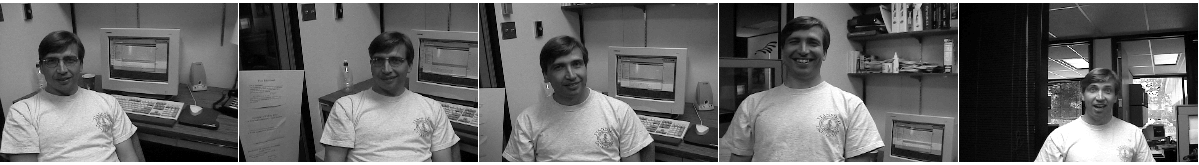
\includegraphics[height=0.95in]{thesis/seq_1_Dudek.png}\label{fig:trk_pca_1a}}
									\subfigure[Davidin300.]{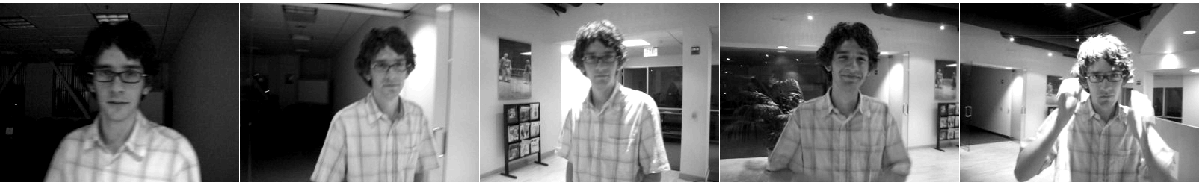
\includegraphics[height=0.95in]{thesis/seq_2_davidin300.png}\label{fig:trk_pca_1b}}
									\subfigure[Sylv.]{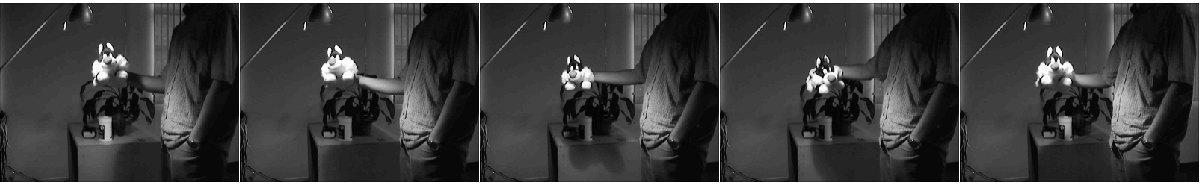
\includegraphics[height=0.95in]{thesis/seq_3_sylv.png}\label{fig:trk_pca_1c}}
									\subfigure[Fish.]{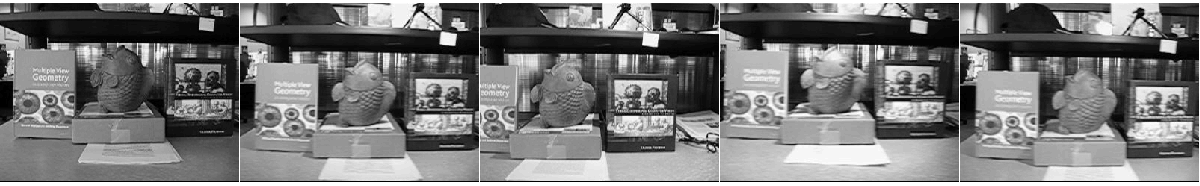
\includegraphics[height=0.95in]{thesis/seq_5_fish.png}\label{fig:trk_pca_1d}}
									\subfigure[Car4.]{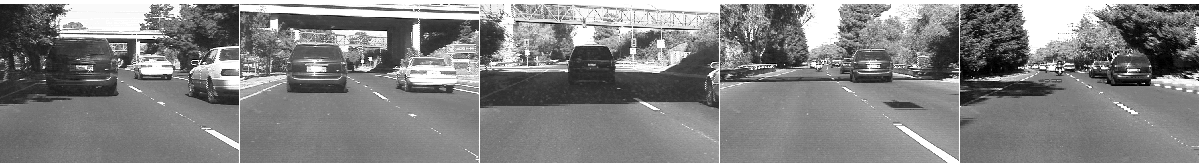
\includegraphics[height=0.95in]{thesis/seq_6_car4.png}\label{fig:trk_pca_1d}}
									\subfigure[Car11.]{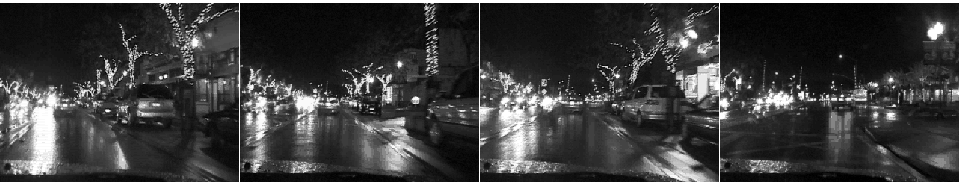
\includegraphics[height=0.95in]{thesis/seq_7_car11.png}\label{fig:trk_pca_1d}}
									\caption{Publicly available tracking sequences downloadable from~\cite{2008_JNL_subspaceTRK_Ross}.}
									\label{fig:trk_sequences}
									\end{figure}


%==========================
\clearpage
\newpage
\section{Tracking error plots}
\label{App:tracking_error_plots}
%==========================
The following 6 pages contain 6 figures corresponding to tracking error plots for PCA, TSVQ, maxP, RofE, nulE and monR based tracking.  Each figure comprises a table and 4 plots.  Each entry in a table represents tracking error temporally averaged over the frames of a dataset (most of the datasets have more than 500 images).  The entries in a table are visualized in the accompanying 4 plots.  The plots show tracking error for different parameter values and their averages, and tracking error for different datasets and their averages. 

%----------------------------------------------------
\clearpage
\newpage
\subsection{PCA}
%----------------------------------------------------
\begin{figure}[h!]
\centering
\begin{tabular}{|l|c|c|c|}
\hline
&\textbf{Q=8}&\textbf{Q=16}&\textbf{Q=32}\\\hline
\textbf{1. Dudek}&7.44&7.81&8.54\\\hline
\textbf{2. davidin300}&8.36&4.60&6.93\\\hline
\textbf{3. sylv}&4.34&5.47&5.72\\\hline
\textbf{4. fish}&9.75&2.17&7.98\\\hline
\textbf{5. car4}&4.79&4.60&5.52\\\hline
\textbf{6. car11}&2.21&2.13&2.39\\\hline
\textbf{mean}&6.15&4.46&6.18\\\hline
\end{tabular}
\\
\subfigure[]{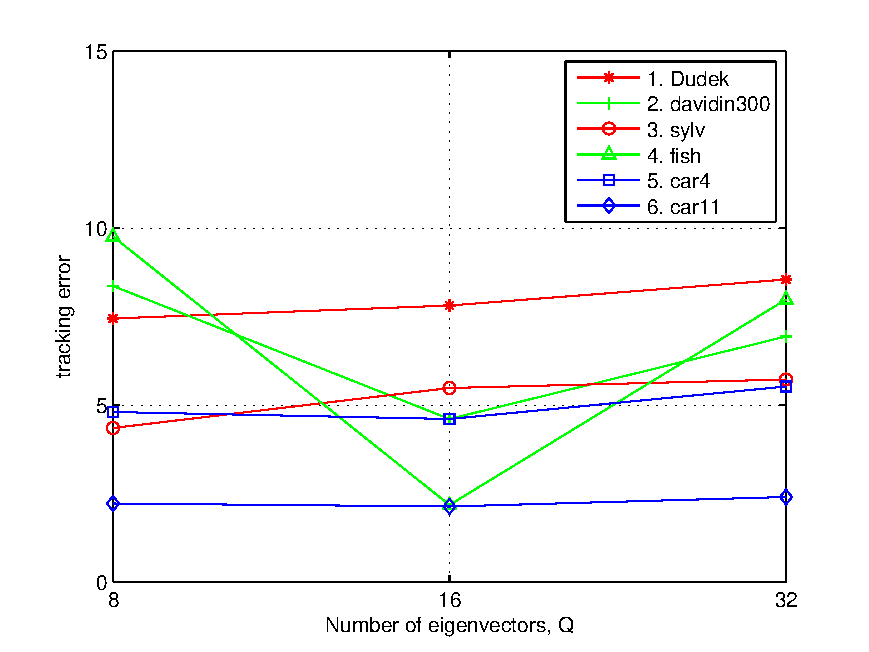
\includegraphics[width=0.45\textwidth]{thesis/results_final_pca__a.pdf}\label{fig:results_final_pca__a}}
\subfigure[]{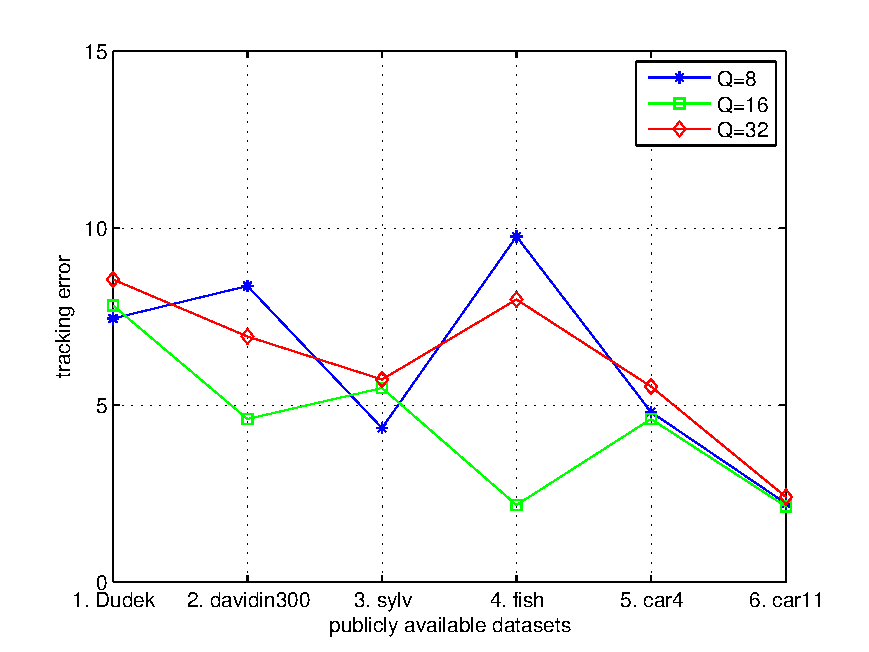
\includegraphics[width=0.45\textwidth]{thesis/results_final_pca__b.pdf}\label{fig:results_final_pca__b}}
\subfigure[]{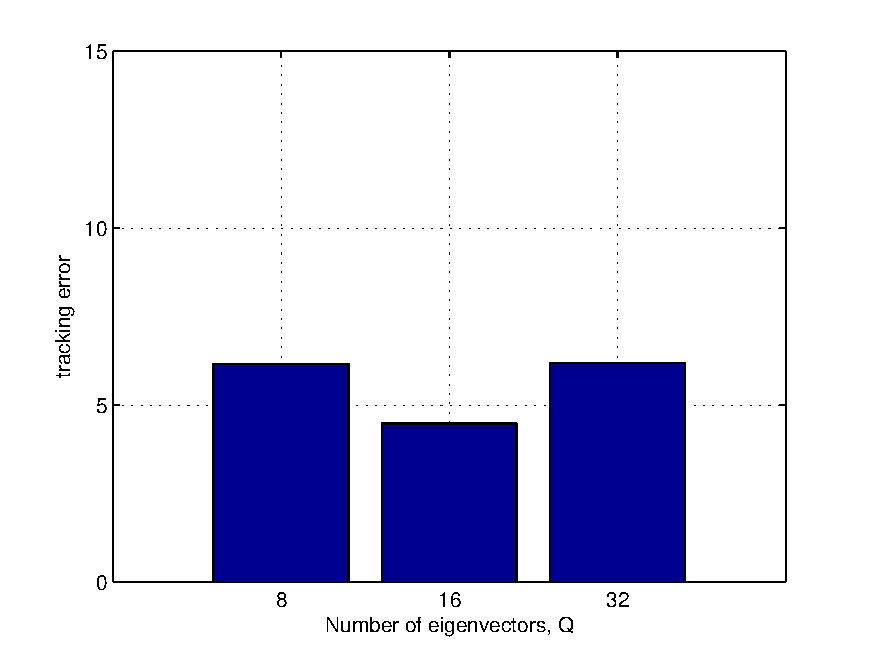
\includegraphics[width=0.45\textwidth]{thesis/results_final_pca__c.pdf}\label{fig:results_final_pca__c}}
\subfigure[]{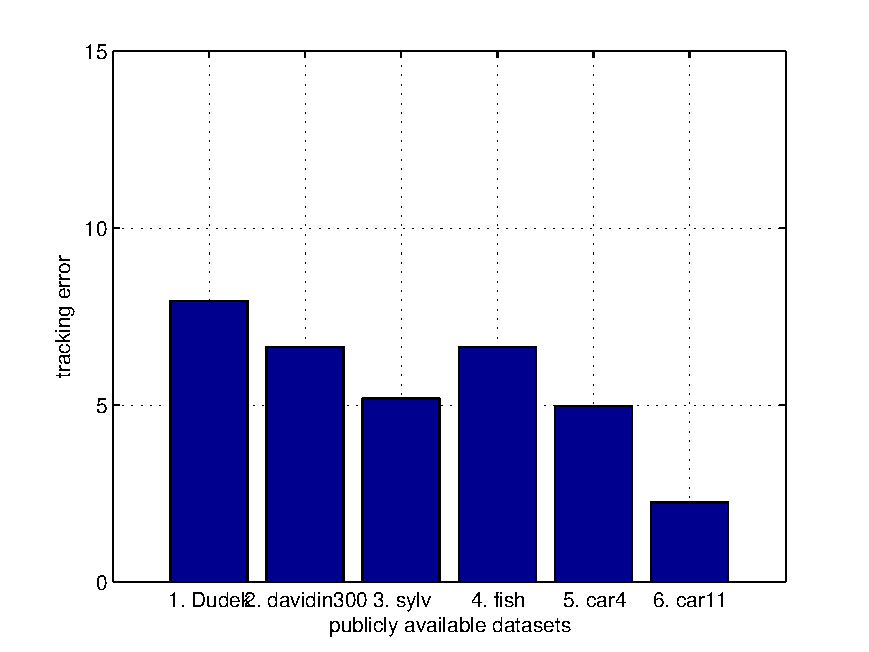
\includegraphics[width=0.45\textwidth]{thesis/results_final_pca__d.pdf}\label{fig:results_final_pca__d}}
\caption{Tracking error for PCA based tracking for different number of eigenvectors $Q$ for 6 different publicly available datasets.}
\label{fig:results_final_pca_}
\end{figure}

%----------------------------------------------------
\clearpage
\newpage
\subsection{TSVQ}
%----------------------------------------------------
\begin{figure}[h!]
\centering
\begin{tabular}{|l|c|c|c|}
\hline
&\textbf{P=3}&\textbf{P=4}&\textbf{P=5}\\\hline
\textbf{1. Dudek}&8.62&11.87&9.71\\\hline
\textbf{2. davidin300}&12.88&6.29&5.93\\\hline
\textbf{3. sylv}&4.70&4.80&4.61\\\hline
\textbf{4. fish}&10.07&4.59&5.47\\\hline
\textbf{5. car4}&5.11&6.79&5.80\\\hline
\textbf{6. car11}&2.21&5.28&2.94\\\hline
\textbf{mean}&7.26&6.60&5.74\\\hline
\end{tabular}
\\
\subfigure[]{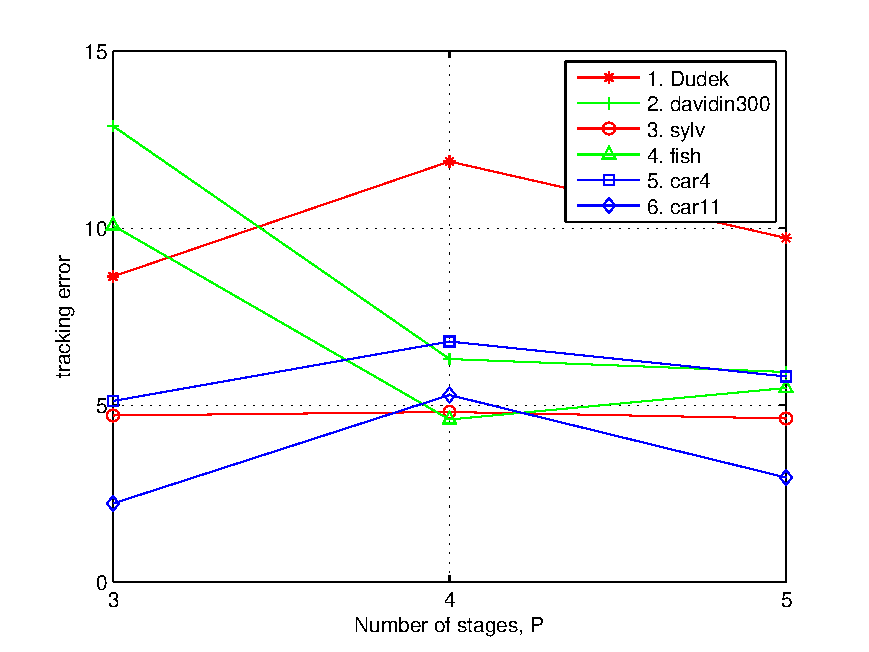
\includegraphics[width=0.45\textwidth]{thesis/results_final_tsvq_a.pdf}\label{fig:results_final_tsvq_a}}
\subfigure[]{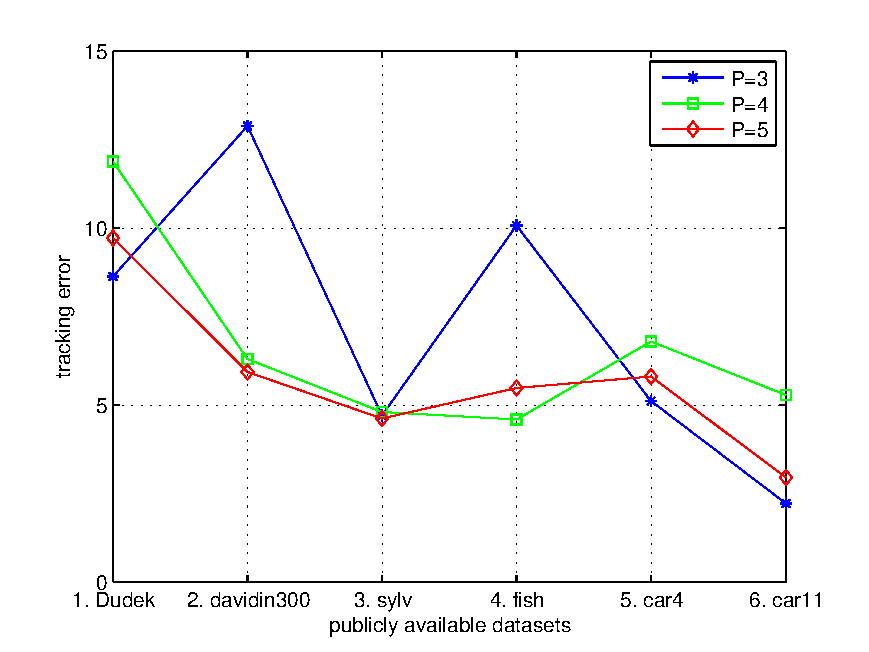
\includegraphics[width=0.45\textwidth]{thesis/results_final_tsvq_b.pdf}\label{fig:results_final_tsvq_b}}
\subfigure[]{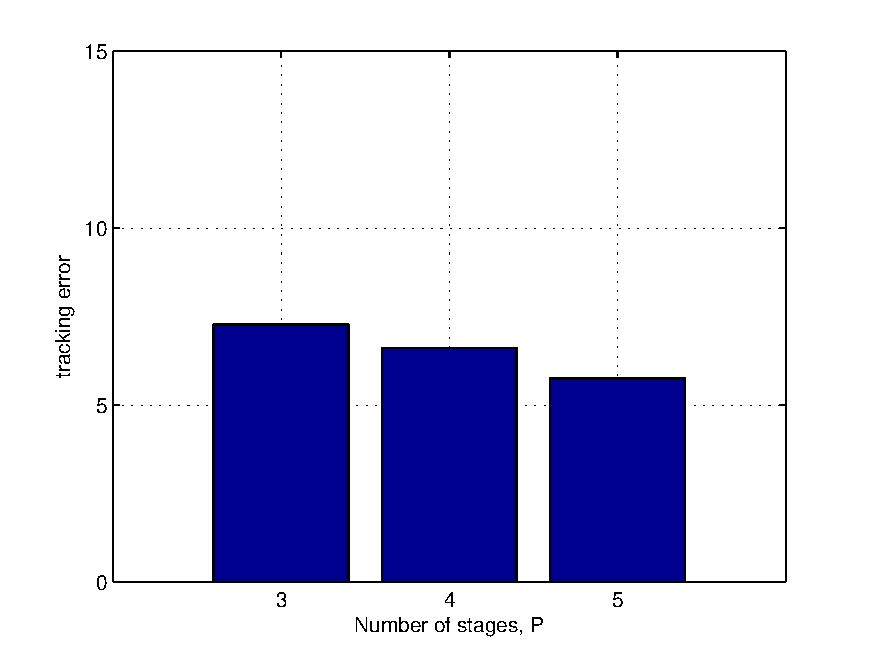
\includegraphics[width=0.45\textwidth]{thesis/results_final_tsvq_c.pdf}\label{fig:results_final_tsvq_c}}
\subfigure[]{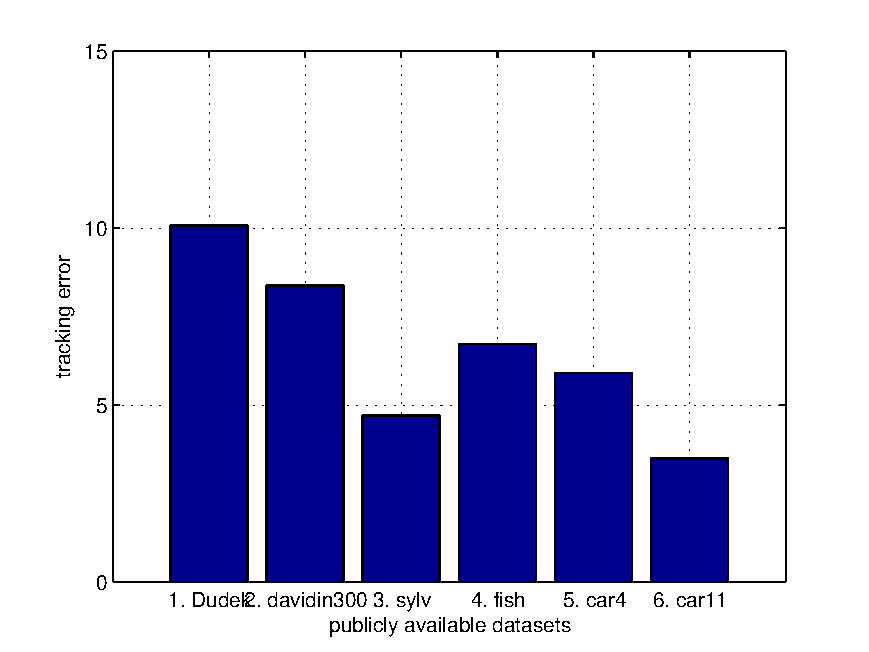
\includegraphics[width=0.45\textwidth]{thesis/results_final_tsvq_d.pdf}\label{fig:results_final_tsvq_d}}
\caption{Tracking error for binary balanced-tree-TSVQ based tracking for different number of stages $P$ for 6 different publicly available datasets.}
\label{fig:results_final_tsvq}
\end{figure}


%----------------------------------------------------
\clearpage
\newpage
\subsection{maxP}
%----------------------------------------------------
\begin{figure}[h!]
\centering
\begin{tabular}{|l|c|c|c|}
\hline
&\textbf{PxM=8x2}&\textbf{PxM=8x4}&\textbf{PxM=8x8}\\\hline
\textbf{1. Dudek}&7.78&7.92&8.09\\\hline
\textbf{2. davidin300}&6.84&4.47&9.89\\\hline
\textbf{3. sylv}&4.00&4.68&4.72\\\hline
\textbf{4. fish}&11.50&2.78&12.15\\\hline
\textbf{5. car4}&4.67&6.38&5.09\\\hline
\textbf{6. car11}&2.17&2.36&3.57\\\hline
\textbf{mean}&6.16&4.76&7.25\\\hline
\end{tabular}
\\
\subfigure[]{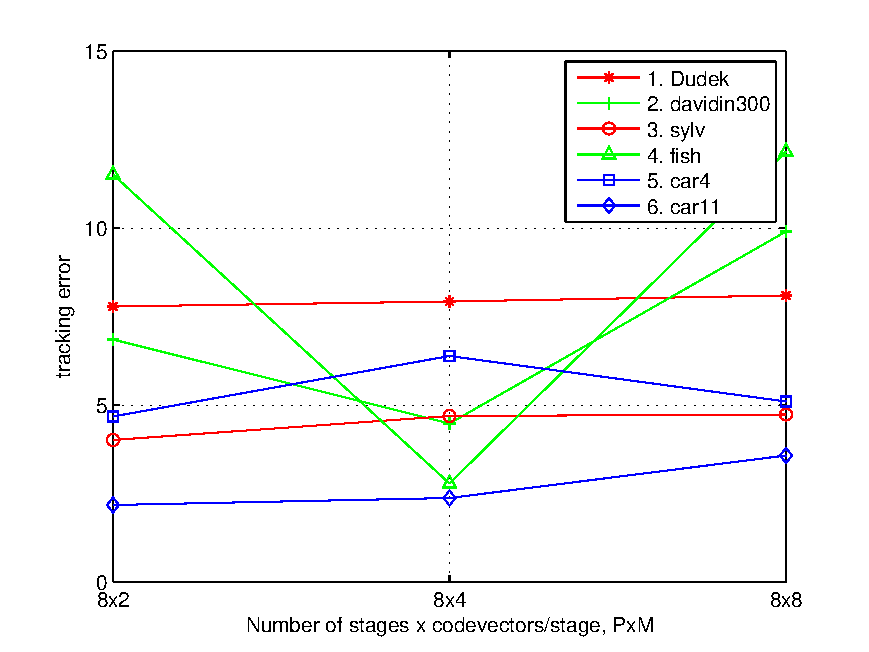
\includegraphics[width=0.45\textwidth]{thesis/results_final_maxP_a.pdf}\label{fig:results_final_maxP_a}}
\subfigure[]{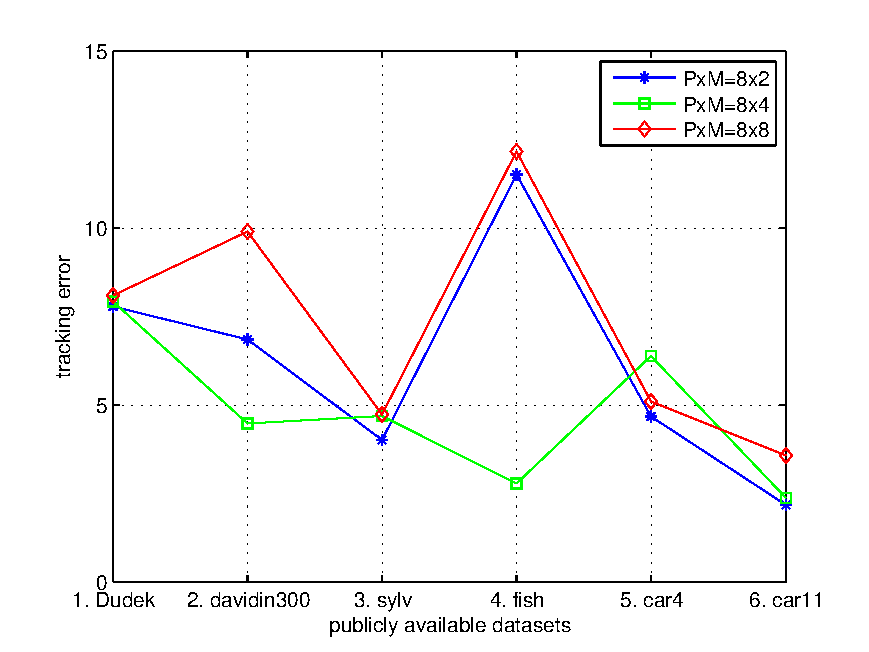
\includegraphics[width=0.45\textwidth]{thesis/results_final_maxP_b.pdf}\label{fig:results_final_maxP_b}}
\subfigure[]{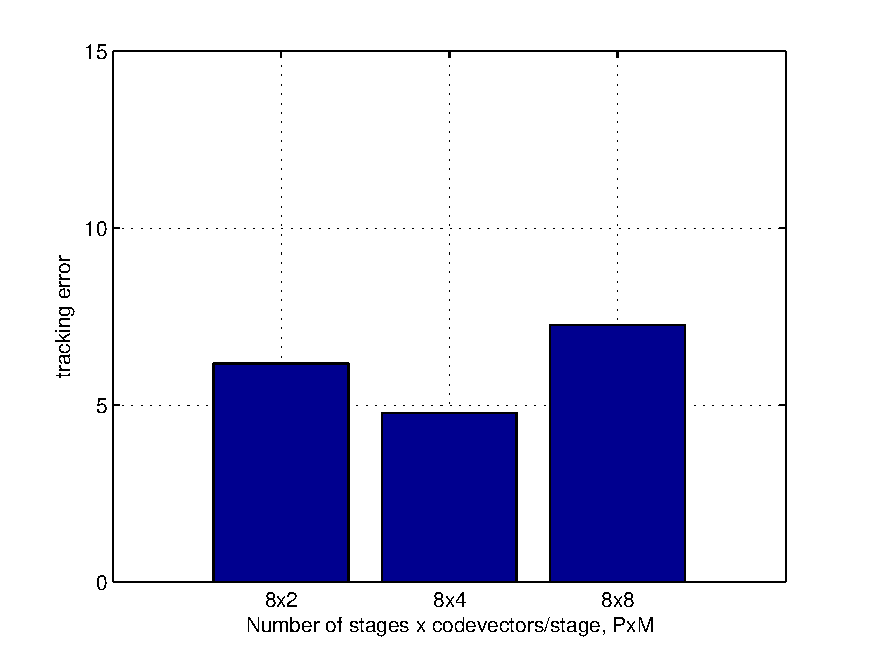
\includegraphics[width=0.45\textwidth]{thesis/results_final_maxP_c.pdf}\label{fig:results_final_maxP_c}}
\subfigure[]{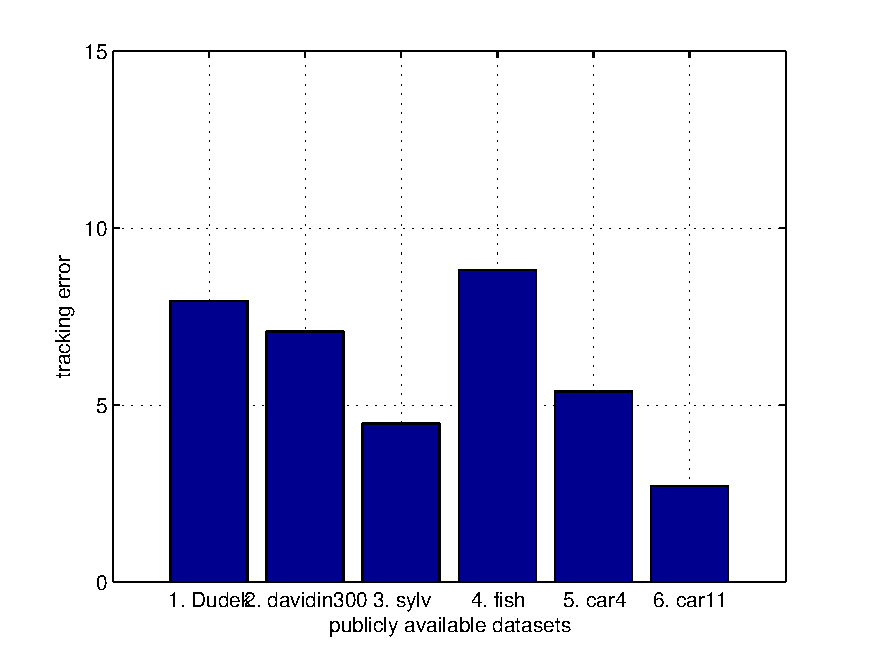
\includegraphics[width=0.45\textwidth]{thesis/results_final_maxP_d.pdf}\label{fig:results_final_maxP_d}}
\caption{Tracking error for maxP based tracking for different number of codevectors per stage $M$ with fixed stages $P=8$ for 6 different publicly available datasets.}
\label{fig:results_final_maxP}
\end{figure}


%----------------------------------------------------
\clearpage
\newpage
\subsection{RofE}
%----------------------------------------------------
\begin{figure}[h!]
\centering
\begin{tabular}{|l|c|c|c|}
\hline
&\textbf{PxM=8x2}&\textbf{PxM=8x4}&\textbf{PxM=8x8}\\\hline
\textbf{1. Dudek}&7.11&8.43&8.19\\\hline
\textbf{2. davidin300}&9.02&6.21&5.74\\\hline
\textbf{3. sylv}&4.12&5.54&4.83\\\hline
\textbf{4. fish}&2.96&12.22&2.73\\\hline
\textbf{5. car4}&4.93&5.14&5.50\\\hline
\textbf{6. car11}&2.47&2.33&2.68\\\hline
\textbf{mean}&5.10&6.64&4.94\\\hline
\end{tabular}
\\
\subfigure[]{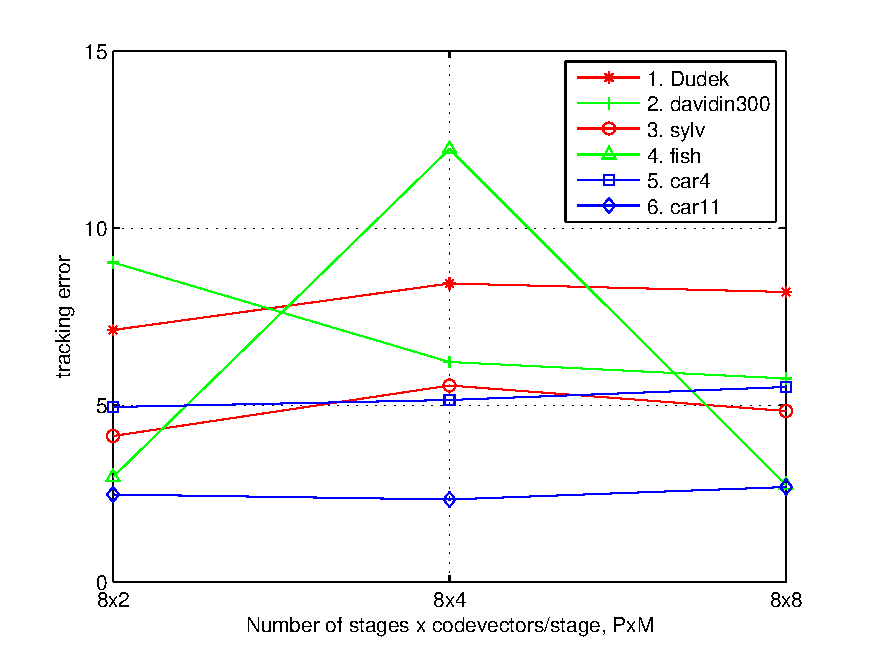
\includegraphics[width=0.45\textwidth]{thesis/results_final_RofE_a.pdf}\label{fig:results_final_RofE_a}}
\subfigure[]{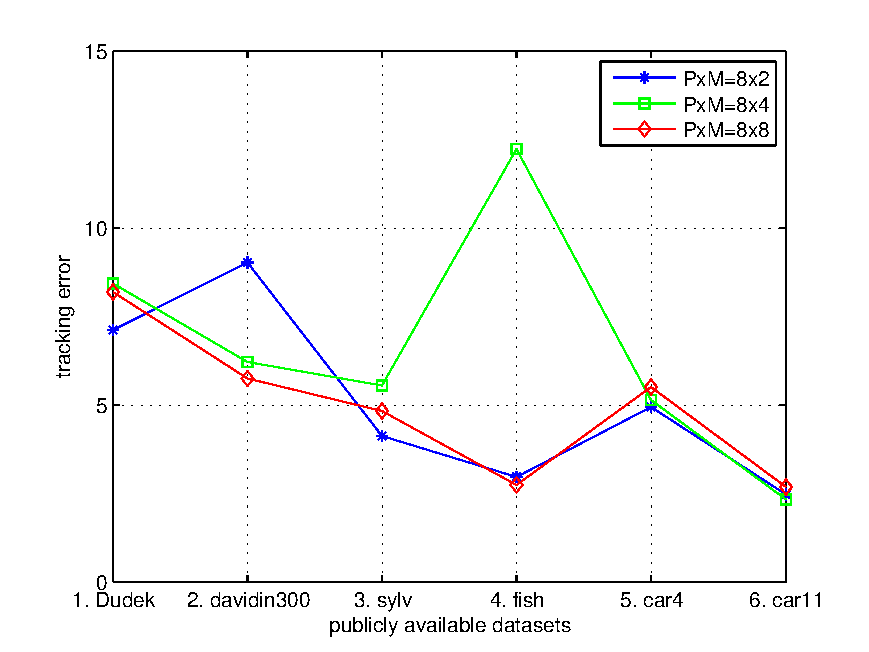
\includegraphics[width=0.45\textwidth]{thesis/results_final_RofE_b.pdf}\label{fig:results_final_RofE_b}}
\subfigure[]{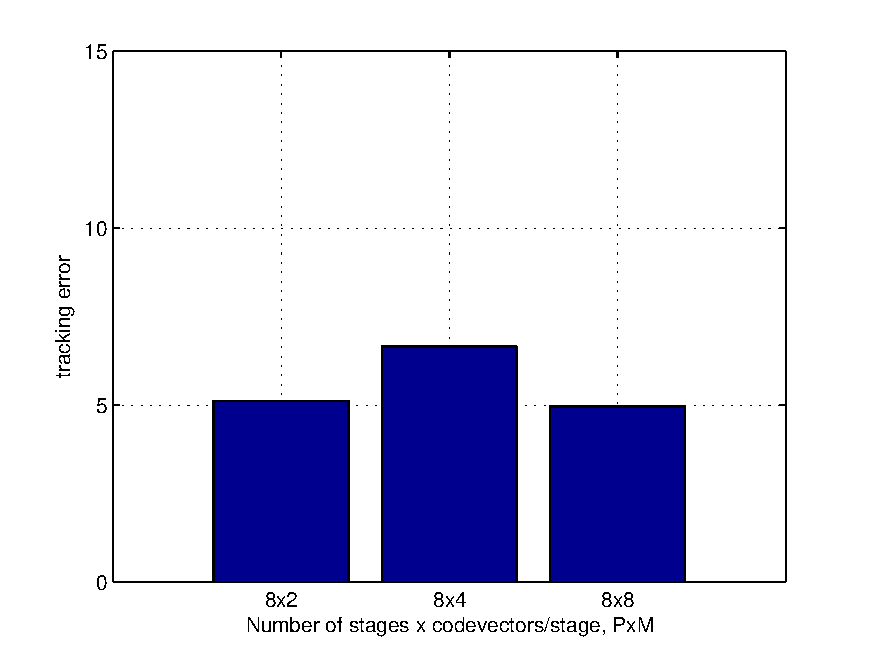
\includegraphics[width=0.45\textwidth]{thesis/results_final_RofE_c.pdf}\label{fig:results_final_RofE_c}}
\subfigure[]{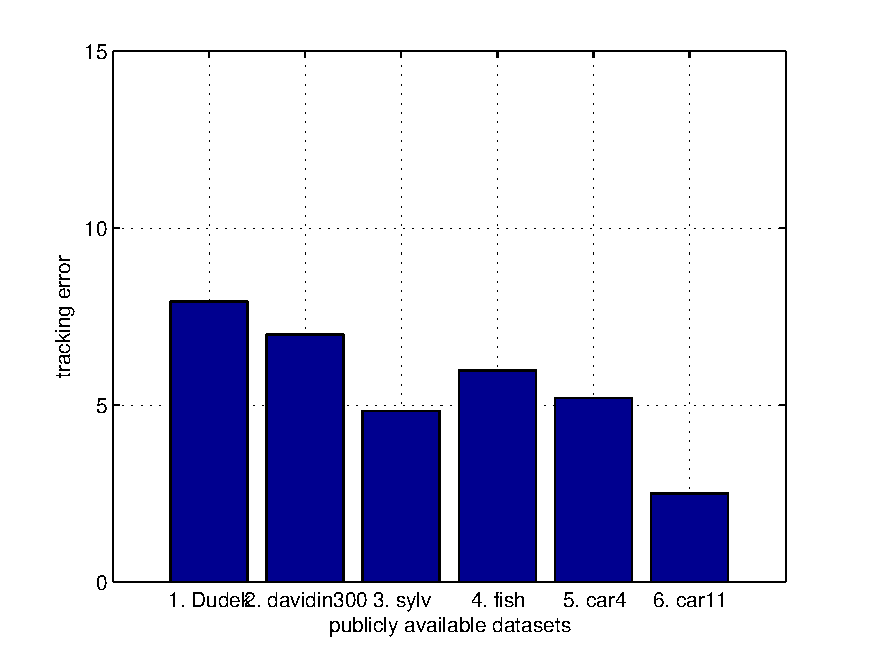
\includegraphics[width=0.45\textwidth]{thesis/results_final_RofE_d.pdf}\label{fig:results_final_RofE_d}}
\caption{Tracking error for RofE based tracking for different number of codevectors per stage $M$ with fixed stages $P=8$ for 6 different publicly available datasets.}
\label{fig:results_final_RofE}
\end{figure}

%----------------------------------------------------
\clearpage
\newpage
\subsection{nulE}
%----------------------------------------------------
\begin{figure}[h!]
\centering
\begin{tabular}{|l|c|c|c|}
\hline
&\textbf{PxM=8x2}&\textbf{PxM=8x4}&\textbf{PxM=8x8}\\\hline
\textbf{1. Dudek}&9.65&8.19&7.97\\\hline
\textbf{2. davidin300}&7.17&5.35&4.63\\\hline
\textbf{3. sylv}&4.81&5.74&4.74\\\hline
\textbf{4. fish}&4.03&2.48&10.71\\\hline
\textbf{5. car4}&5.28&5.84&6.19\\\hline
\textbf{6. car11}&2.59&2.52&2.96\\\hline
\textbf{mean}&5.59&5.02&6.20\\\hline
\end{tabular}
\\
\subfigure[]{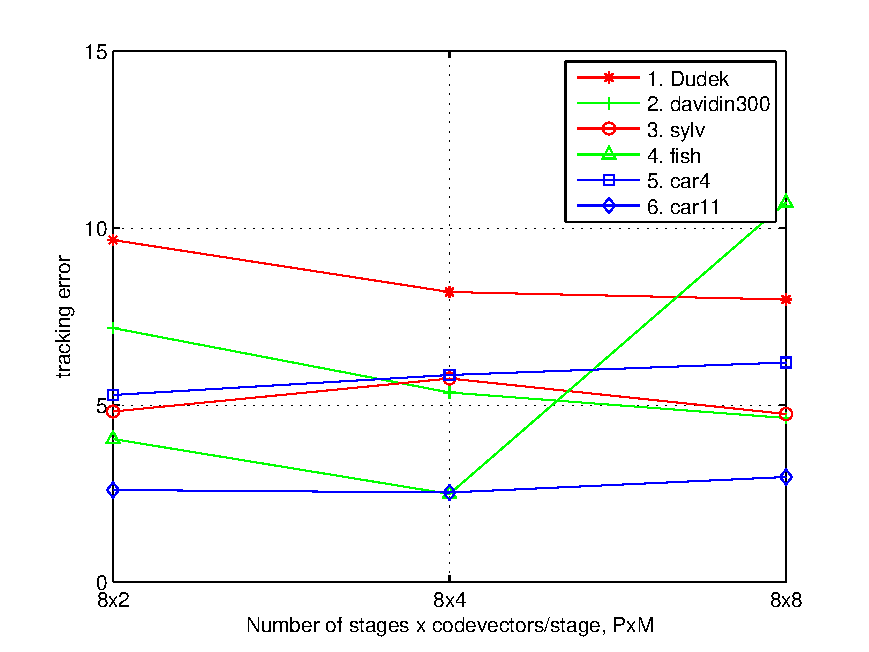
\includegraphics[width=0.45\textwidth]{thesis/results_final_nulE_a.pdf}\label{fig:results_final_nulE_a}}
\subfigure[]{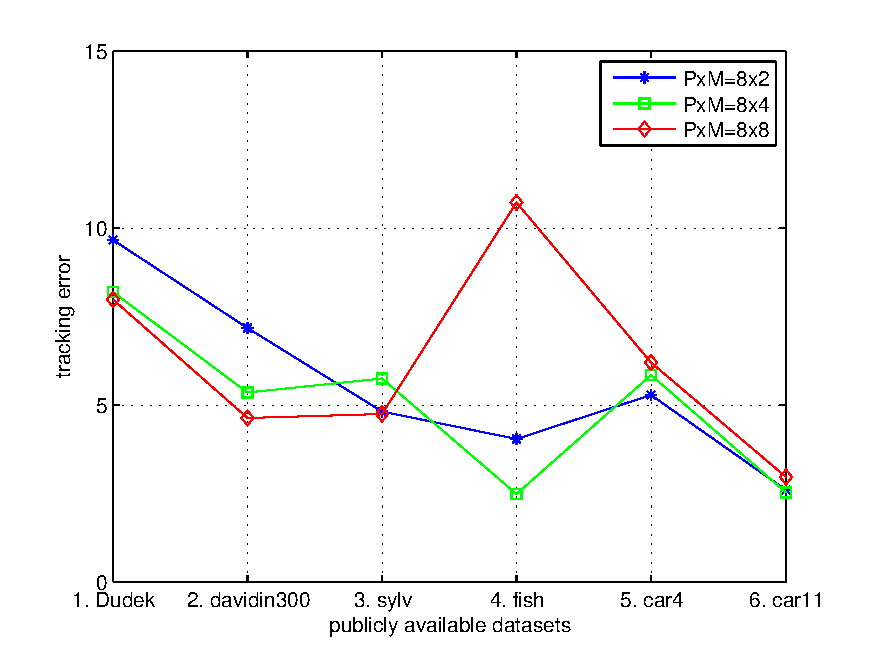
\includegraphics[width=0.45\textwidth]{thesis/results_final_nulE_b.pdf}\label{fig:results_final_nulE_b}}
\subfigure[]{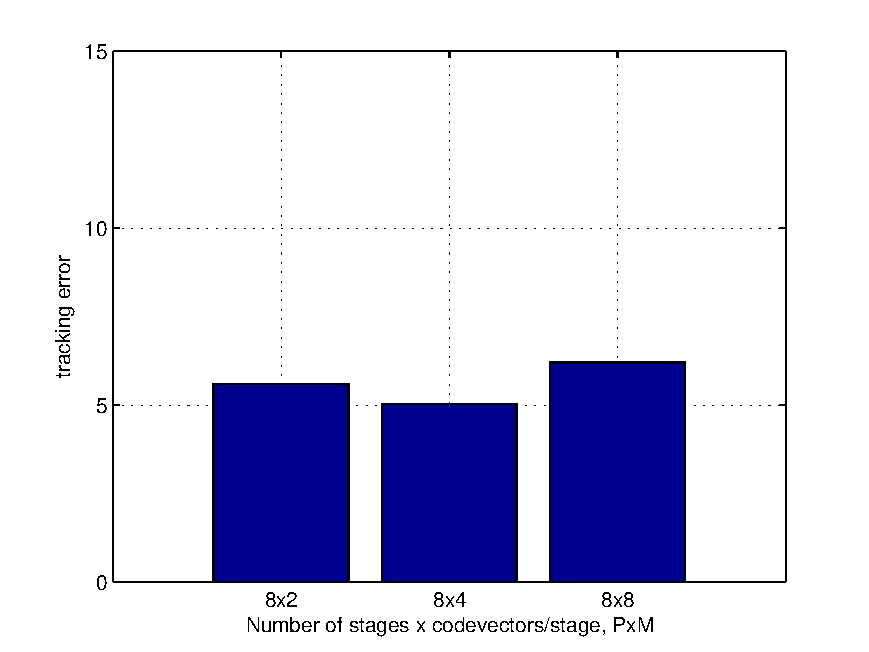
\includegraphics[width=0.45\textwidth]{thesis/results_final_nulE_c.pdf}\label{fig:results_final_nulE_c}}
\subfigure[]{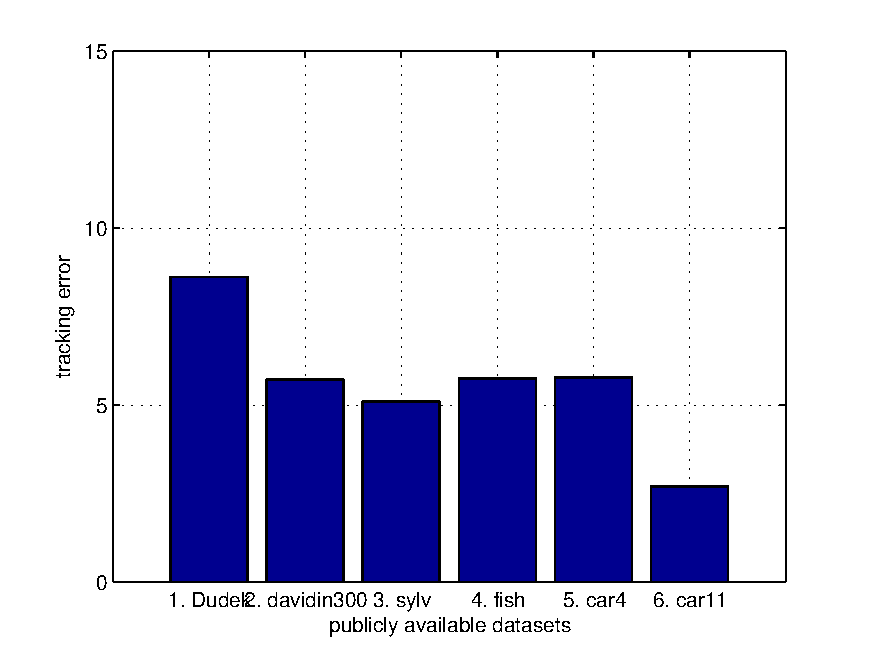
\includegraphics[width=0.45\textwidth]{thesis/results_final_nulE_d.pdf}\label{fig:results_final_nulE_d}}
\caption{Tracking error for nulE based tracking for different number of codevectors per stage $M$ with fixed stages $P=8$ for 6 different publicly available datasets.}
\label{fig:results_final_nulE}
\end{figure}
%----------------------------------------------------
\clearpage
\newpage
\subsection{monR}
%----------------------------------------------------
\begin{figure}[h!]
\centering
\begin{tabular}{|l|c|c|c|}
\hline
&\textbf{PxM=8x2}&\textbf{PxM=8x4}&\textbf{PxM=8x8}\\\hline
\textbf{1. Dudek}&11.81&9.17&8.73\\\hline
\textbf{2. davidin300}&50.00&5.83&4.15\\\hline
\textbf{3. sylv}&4.31&4.58&5.08\\\hline
\textbf{4. fish}&2.89&3.62&11.94\\\hline
\textbf{5. car4}&5.07&5.18&4.71\\\hline
\textbf{6. car11}&2.47&2.72&2.55\\\hline
\textbf{mean}&5.31&5.18&6.19\\\hline
\end{tabular}
\\
\subfigure[]{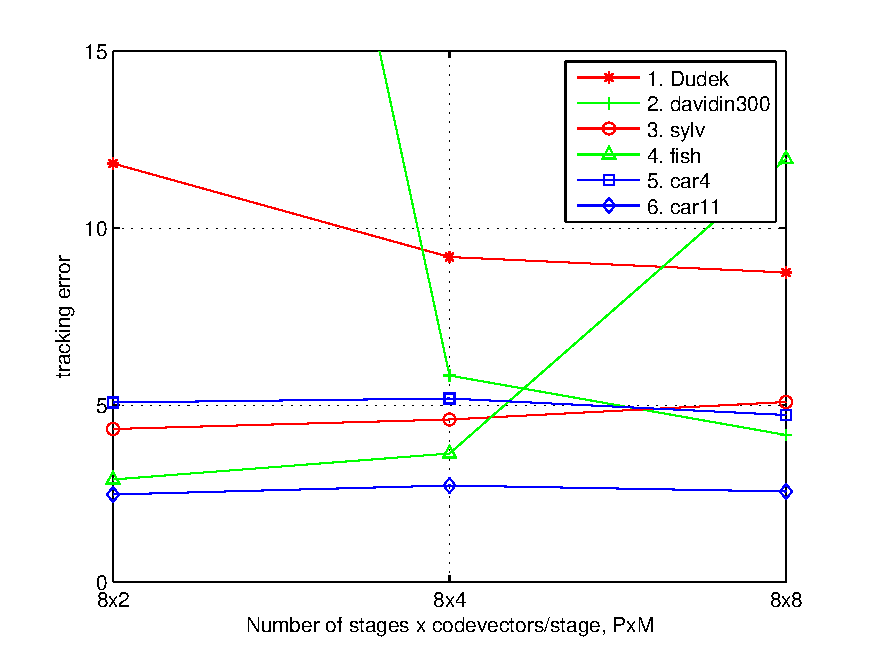
\includegraphics[width=0.45\textwidth]{thesis/results_final_monR_a.pdf}\label{fig:results_final_monR_a}}
\subfigure[]{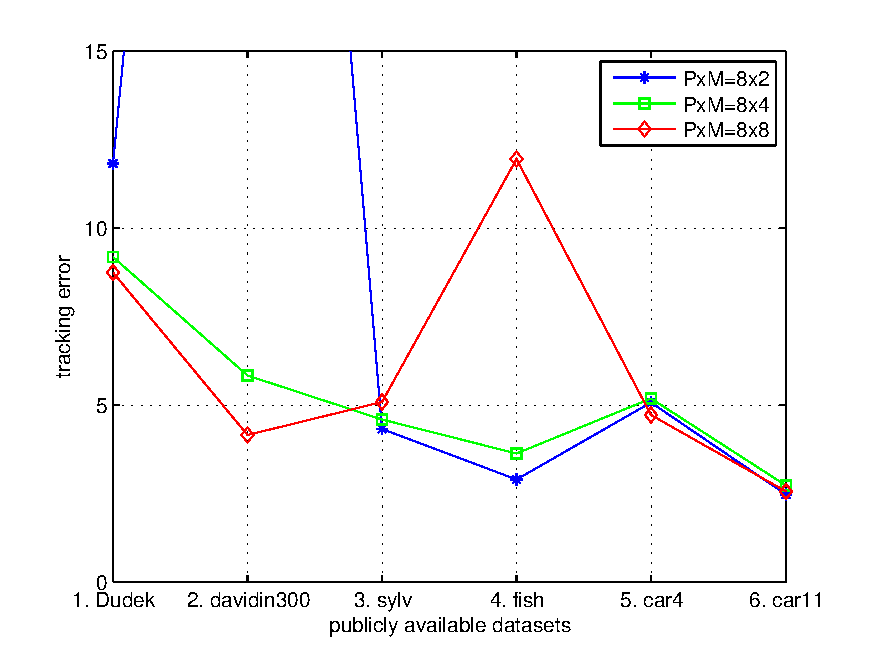
\includegraphics[width=0.45\textwidth]{thesis/results_final_monR_b.pdf}\label{fig:results_final_monR_b}}
\subfigure[]{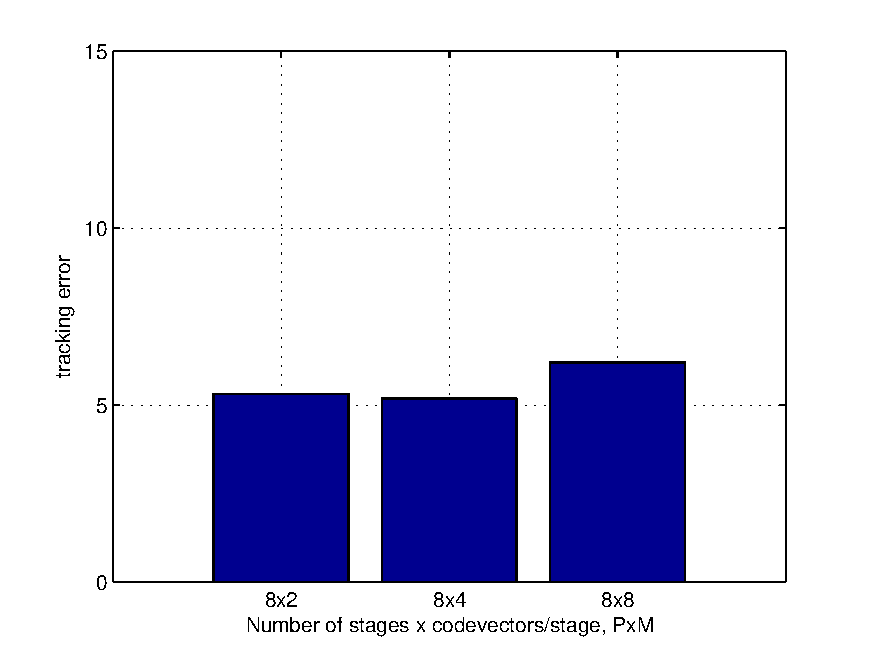
\includegraphics[width=0.45\textwidth]{thesis/results_final_monR_c.pdf}\label{fig:results_final_monR_c}}
\subfigure[]{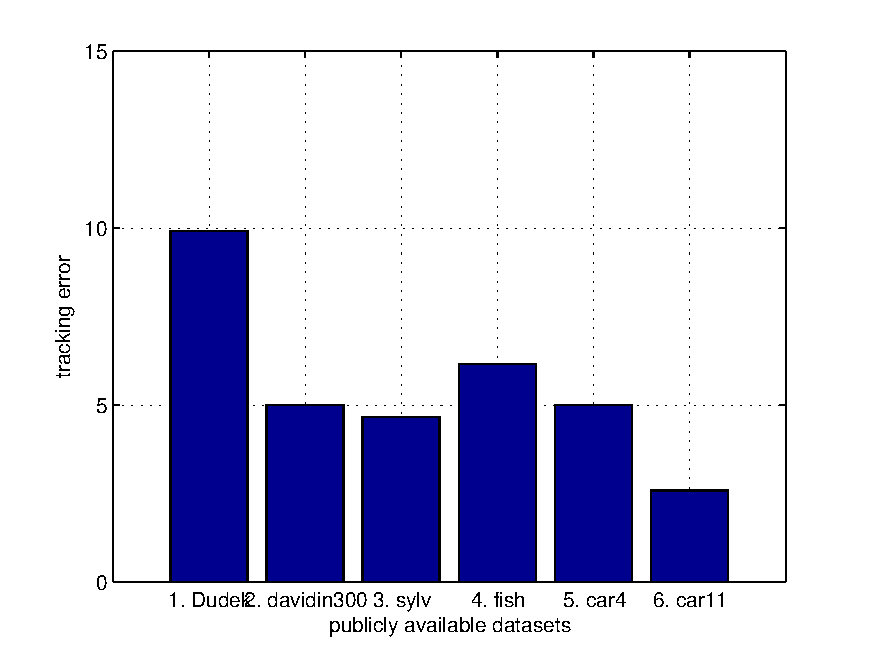
\includegraphics[width=0.45\textwidth]{thesis/results_final_monR_d.pdf}\label{fig:results_final_monR_d}}
\caption{Tracking error for monR based tracking for different number of codevectors per stage $M$ with fixed stages $P=8$ for 6 different publicly available datasets. A value of 50 means that track was lost.  The computation of the mean ignores the lost track case.}
\label{fig:results_final_monR}
\end{figure}

%==========================
\clearpage
\newpage
\section{Example of tracking error}
\label{App:TSVQ_Dudek_example}
%==========================
\begin{figure}[h!]
\centering
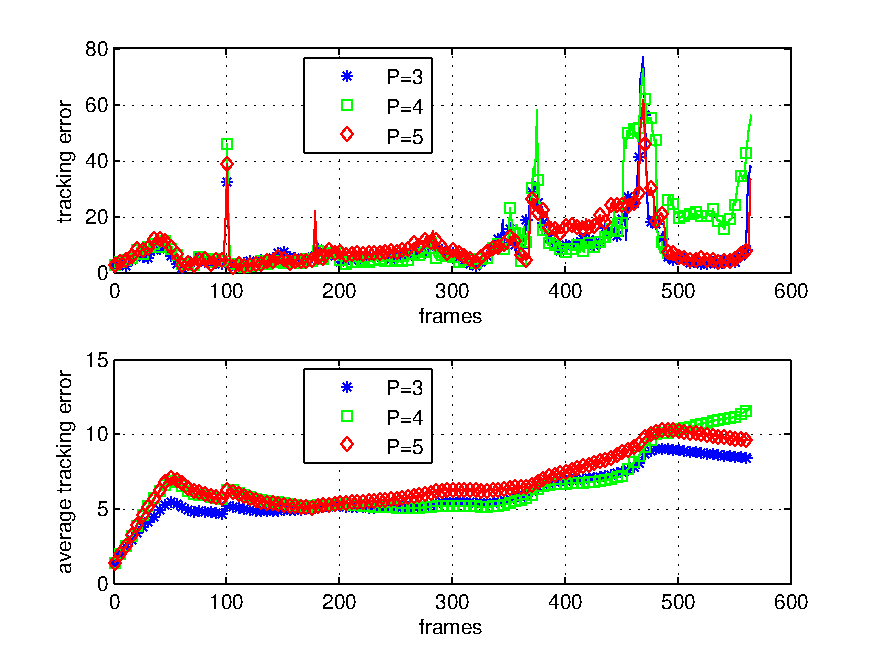
\includegraphics[width=1.0\textwidth]{thesis/Dudek_TSVQ_errors.pdf}
\caption{Tracking error for TSVQ tracker, $P$=3, 4, 5, Dudek sequence.  The top figure shows instantaneous tracking error for the current frame while the bottom figure shows average tracking errors.  Notice that at frame 457, the tracker with $P=4$ makes an error which causes its average error to first exceed that of the $P$=2 tracker, and then eventually the $P$=5 tracker.}
\label{fig:results_TSVQ_Dudek_errors}
\end{figure}

\begin{figure}[h!]
\centering
\subfigure[Ground truth.]{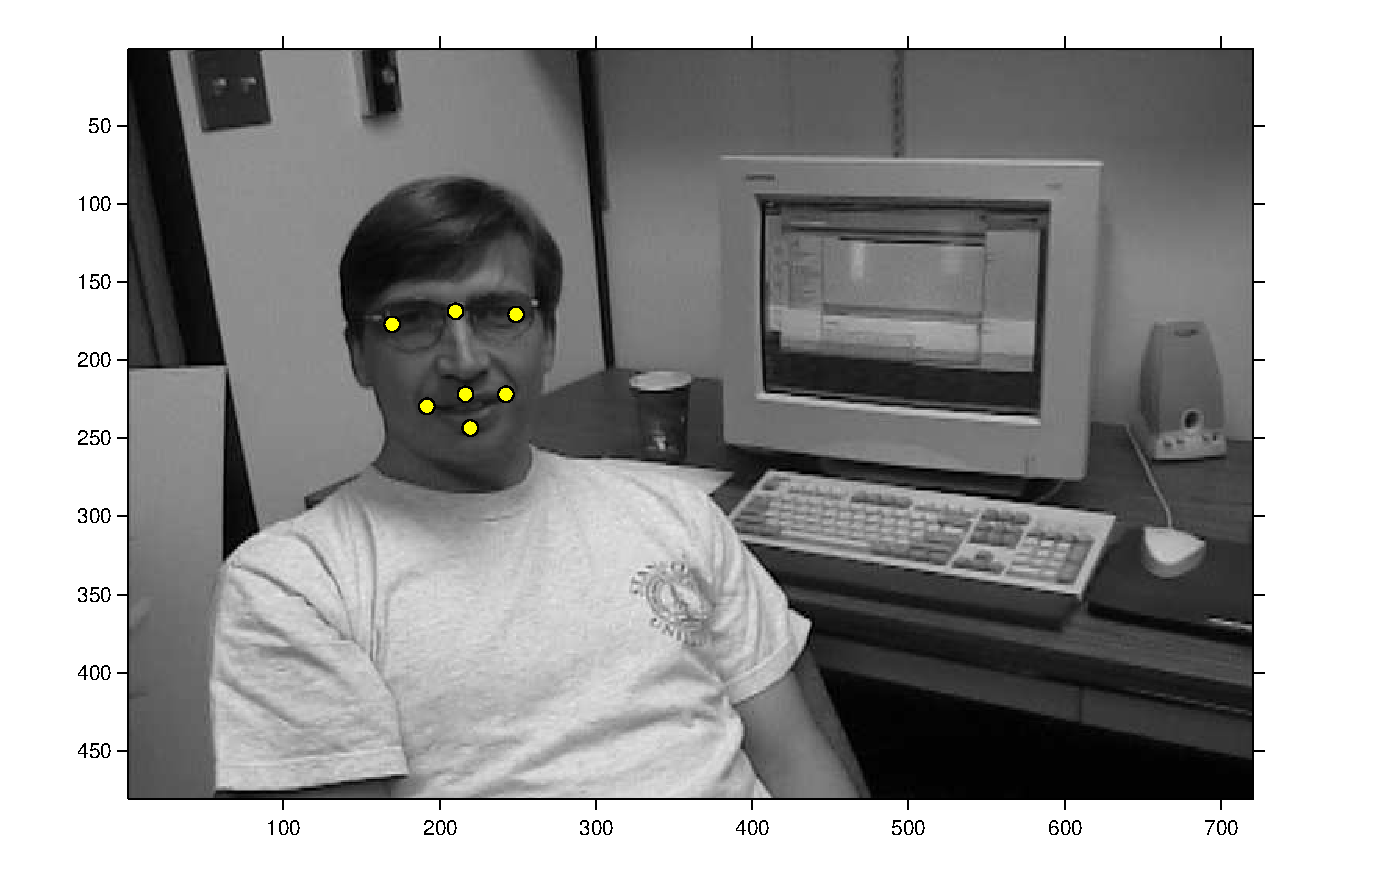
\includegraphics[width=0.3\textwidth]{thesis/Dudek_GT_FN10.pdf}\label{fig:results_final_monR_b}}
\subfigure[$P$=3.]{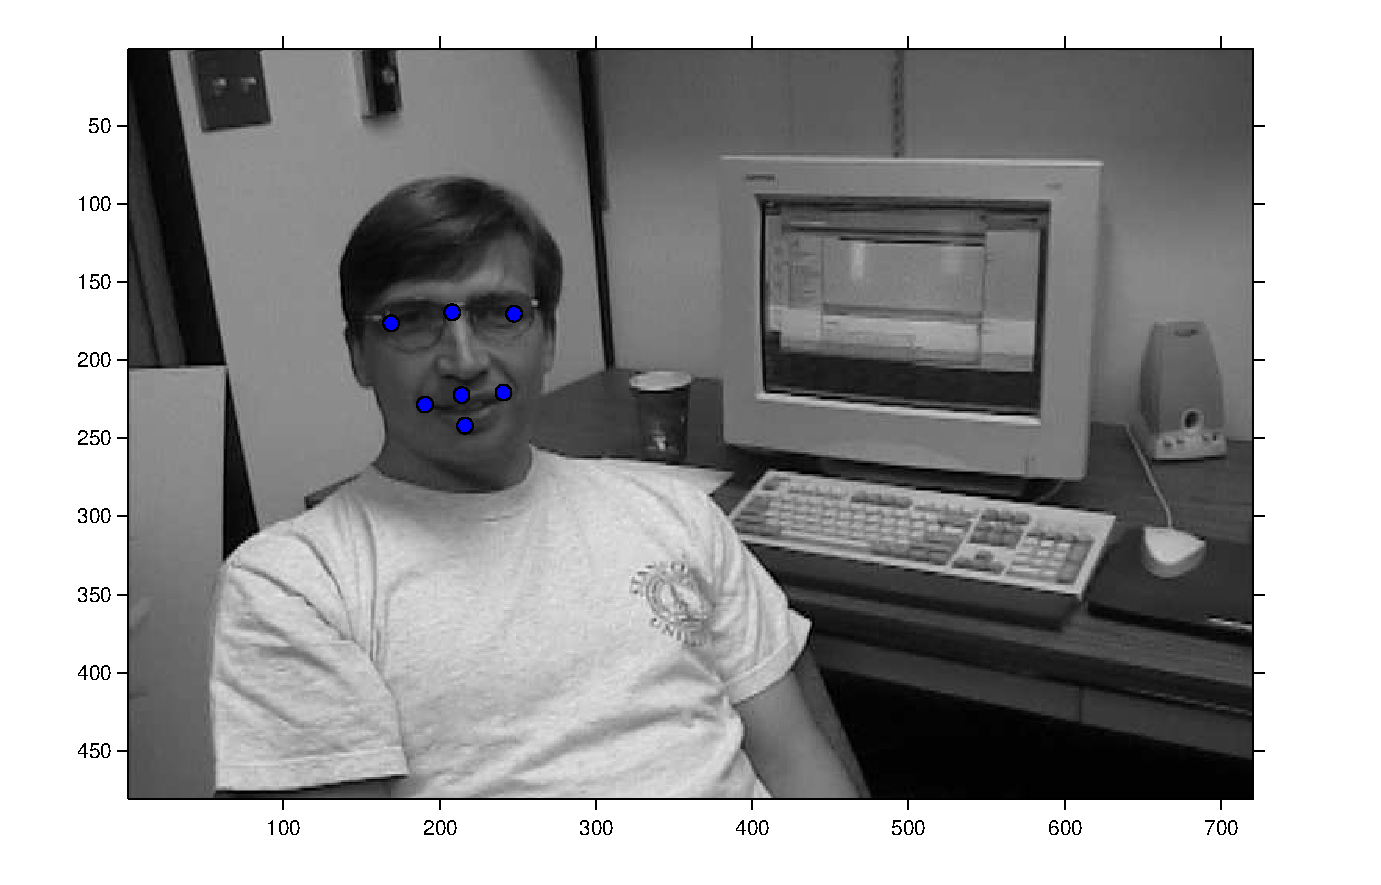
\includegraphics[width=0.3\textwidth]{thesis/Dudek_TSVQ_FN10_P3.pdf}\label{fig:Dudek_TSVQ_FN10_P3}}
\subfigure[$P$=4.]{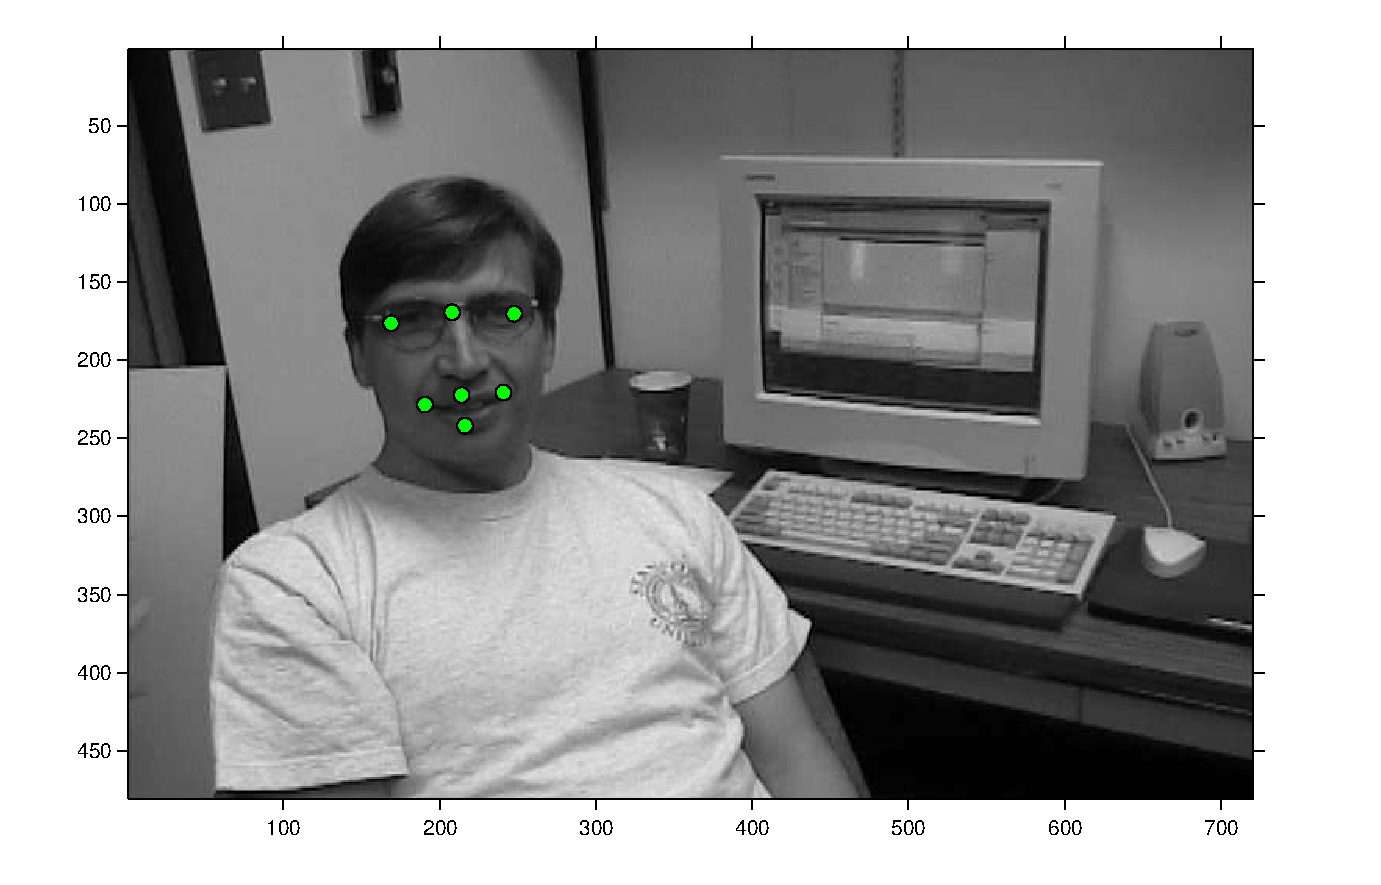
\includegraphics[width=0.3\textwidth]{thesis/Dudek_TSVQ_FN10_P4.pdf}\label{fig:Dudek_TSVQ_FN10_P4}}
\subfigure[$P$=5.]{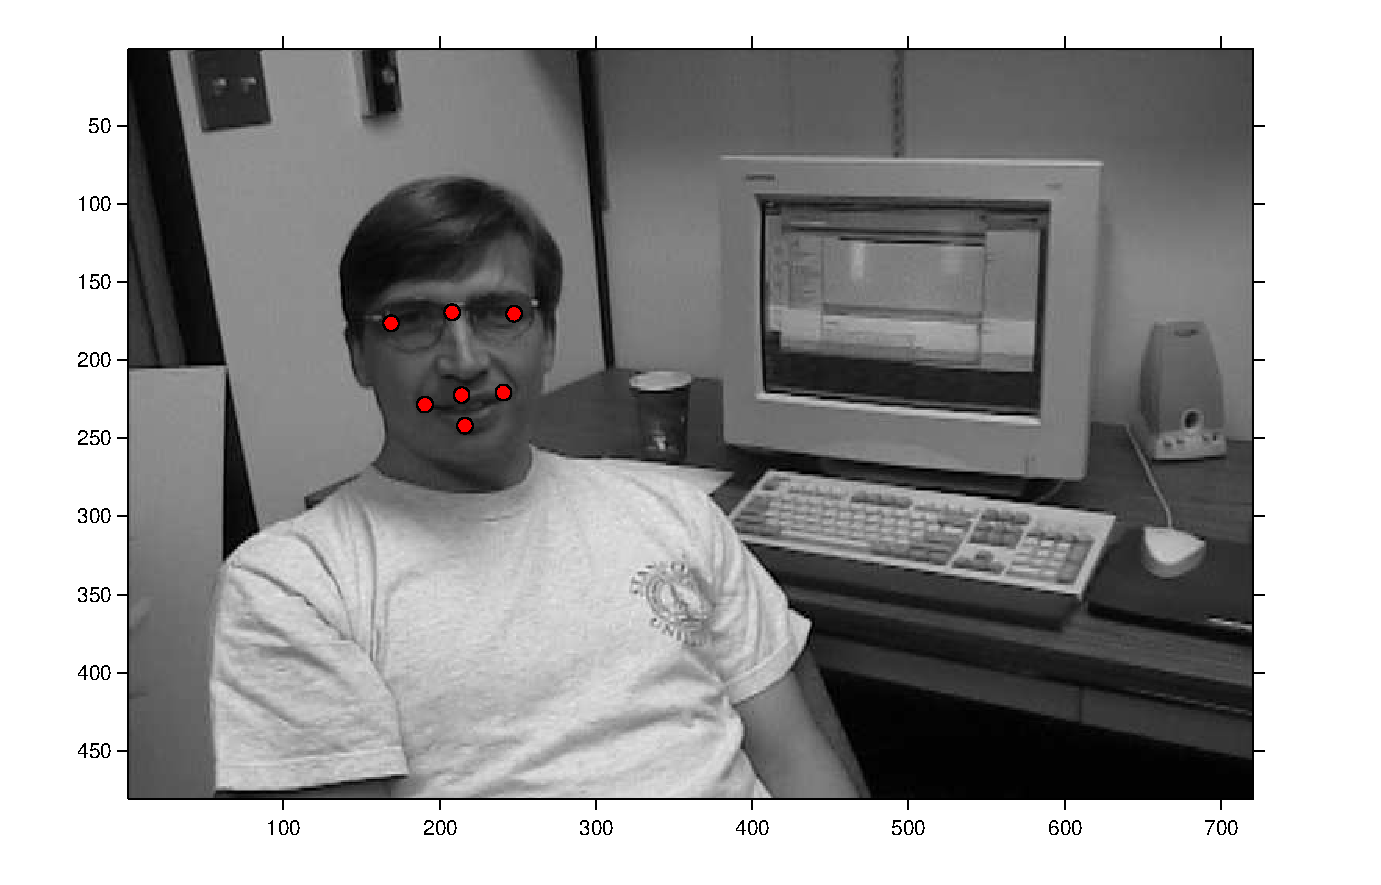
\includegraphics[width=0.3\textwidth]{thesis/Dudek_TSVQ_FN10_P5.pdf}\label{fig:Dudek_TSVQ_FN10_P5}}
\caption{Low tracking error for TSVQ tracker, frame number=10.  The overlaid circles are ground truth and estimated feature points.}
\label{fig:results_TSVQ_Dudek_FN10}
\end{figure}


\begin{figure}[h!]
\centering
\subfigure[Ground truth.]{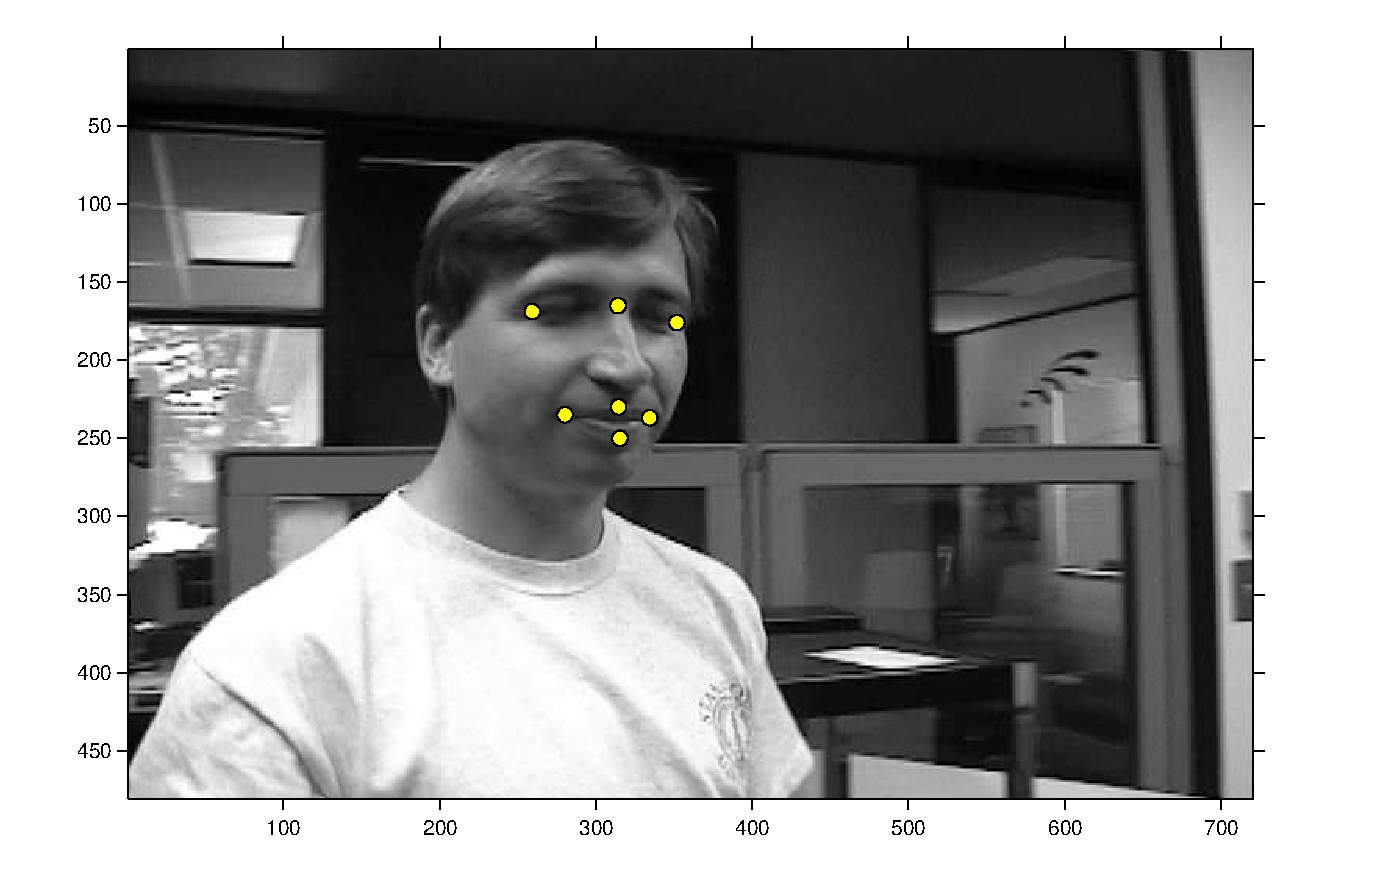
\includegraphics[width=0.3\textwidth]{thesis/Dudek_GT_FN457.pdf}\label{fig:results_final_monR_b}}
\subfigure[$P$=3.]{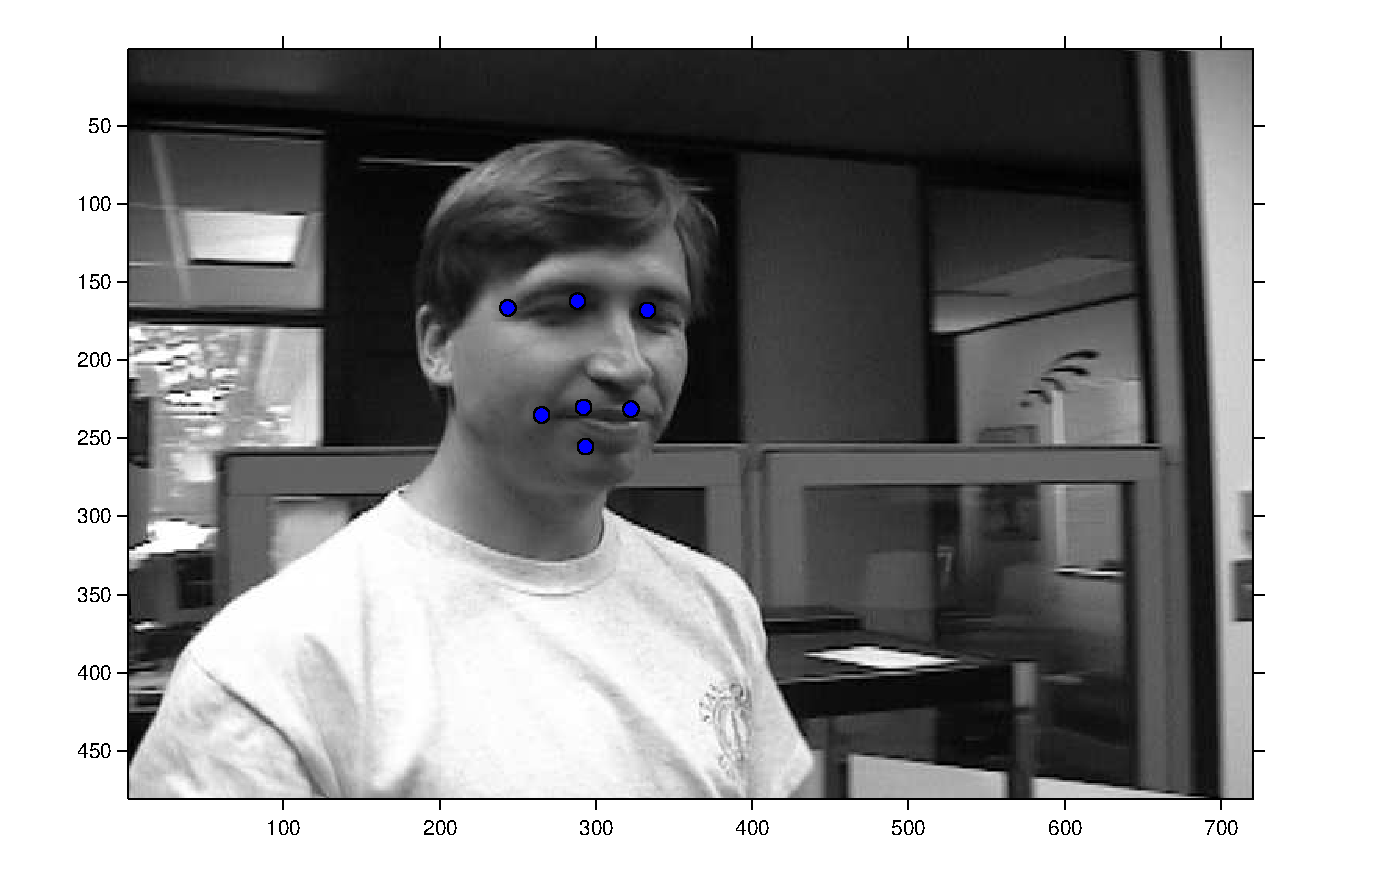
\includegraphics[width=0.3\textwidth]{thesis/Dudek_TSVQ_FN457_P3.pdf}\label{fig:Dudek_TSVQ_FN10_P3}}
\subfigure[$P$=4.]{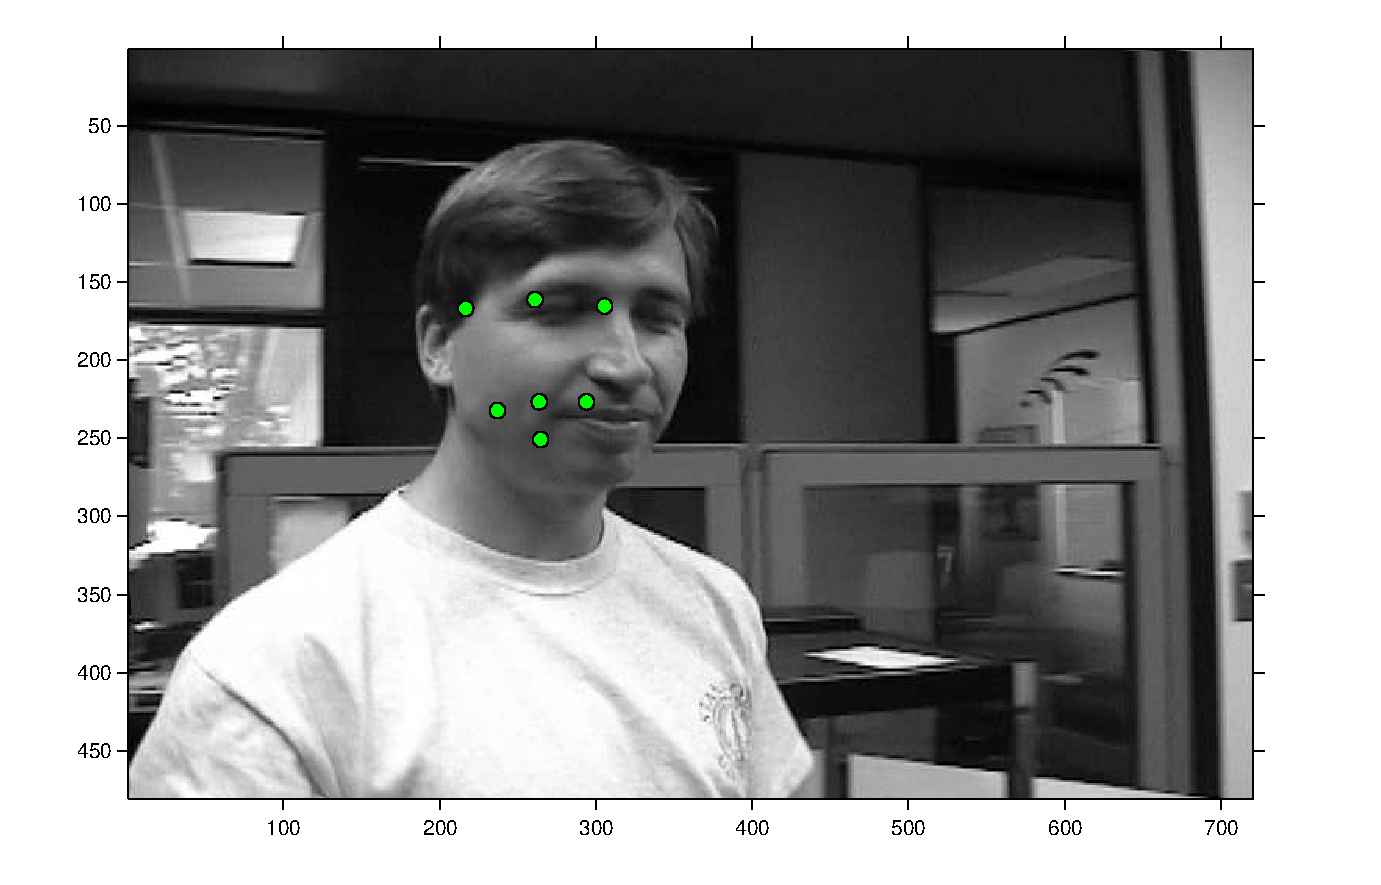
\includegraphics[width=0.3\textwidth]{thesis/Dudek_TSVQ_FN457_P4.pdf}\label{fig:Dudek_TSVQ_FN10_P4}}
\subfigure[$P$=5.]{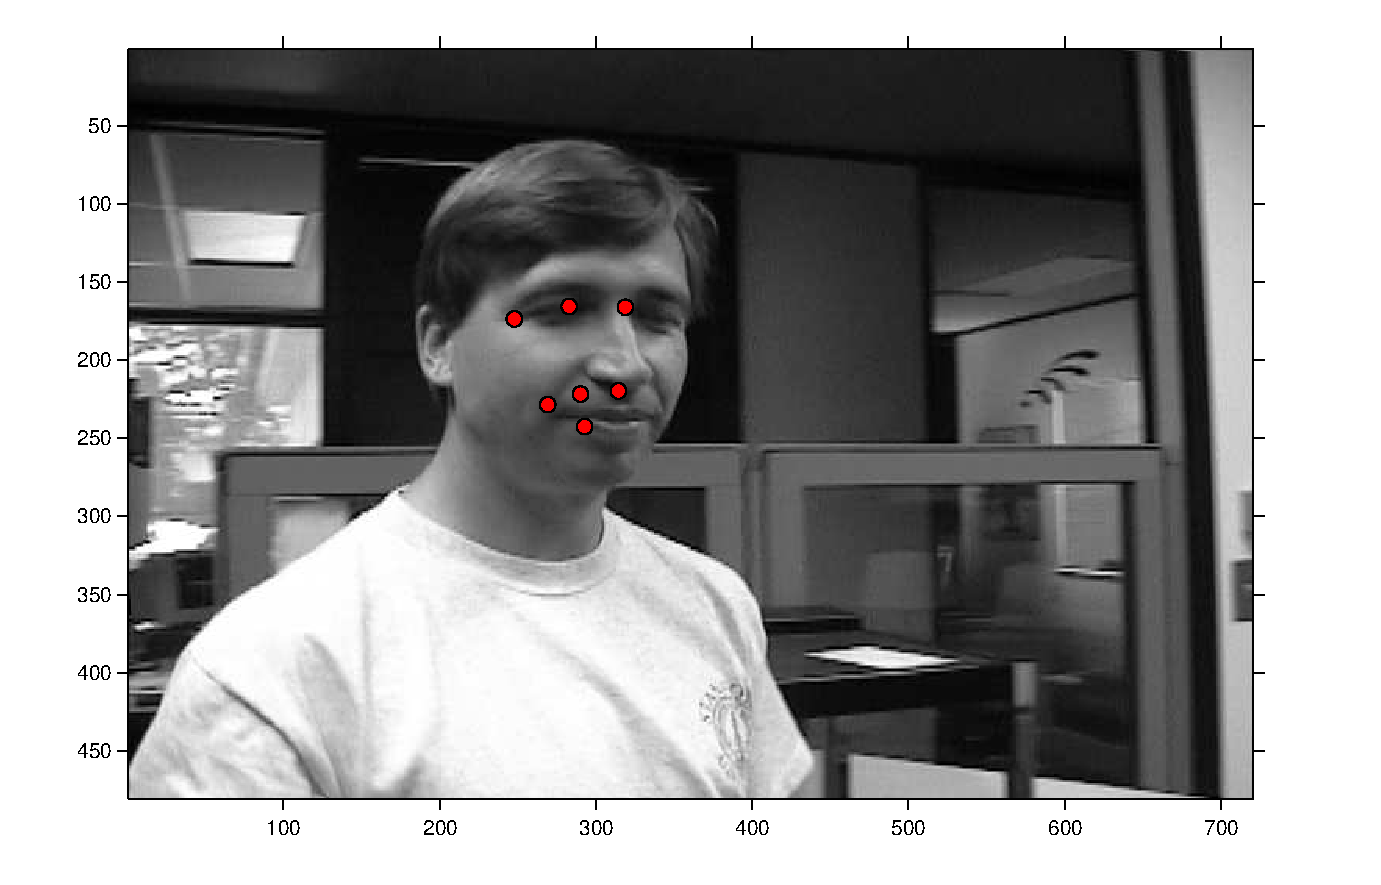
\includegraphics[width=0.3\textwidth]{thesis/Dudek_TSVQ_FN457_P5.pdf}\label{fig:Dudek_TSVQ_FN10_P5}}
\caption{High tracking error for TSVQ tracker, frame number=457.  In this frame, the person being tracked is swiftly turning his head and moving at the same time.  The tracking errors for $P$=3, 4 and 5 are 19.9, 47.3 and 25.1 respectively.  This error causes average error for $P$=4 to first exceed that of the $P$=2 tracker, and then eventually the $P$=5 tracker.  This shows that an error at a time when the target is undergoing large motion can be costly in the long term.  This is because a wrong decision can cause the wrong snippet to be included in the training set which can cause further wrong decisions.}
\label{fig:results_TSVQ_Dudek_FN457}
\end{figure}
